\documentclass{article}
\usepackage{braille}
\usepackage{fontspec}
\newfontfamily{\braille}{DejaVu Serif}

\begin{document}
{\obeylines\braille
⡂⡀⣀⢀⣄⡀⣰⡉⡀⠀⡀⡀⣀⠀⢀⣀⢀⣄⡀⡂⢀⣀⡀⢀⢀⡀⠀⡰⣀⠀⣀⠀⡂⡀⣀⢀⣄⡰⡀⢠⠂
⡇⡏⠀⡇⡇⠀⢸⠀⡇⢀⡇⡏⠀⡇⣏⠀⠀⡇⠀⡇⣏⠀⣹⢸⠁⢸⠀⡇⢈⠷⡁⠀⡇⡏⠀⡇⡇⠀⡇⢼⠀
⠁⠁⠀⠁⠈⠁⠈⠀⠈⠁⠁⠁⠀⠁⠈⠉⠀⠈⠁⠁⠈⠉⠁⠈⠀⠈⠀⠱⠉⠀⠉⠀⠁⠁⠀⠁⠈⠱⠁⠘⠄
⠀⠀⠀⠀⠀⠀⠀⠀⠀⠀⠀⠀⠀⠀⠀⠀⠀⠀⠀⠀⠀⠀⠀⠀⠀⠀⠀⠀⠀⠀⠀⠀⠀⠀⠀⠀⠀⠀⠀⠀⠀
⠀⠀⠀⢤⡀⡤⠀⣀⣀⣀⠀⢤⡀⡤⠀⠀⢰⠀⠀⢹⠠⠀
⠀⠀⠀⣠⠛⣄⠀⠒⠒⠒⠀⣠⠛⣄⠀⠉⢹⠉⠁⢸⢀⠀
⠀⠀⠀⠀⠀⠀⠀⠀⠀⠀⠀⠀⠀⠀⠀⠀⠀⠀⠀⠀⠘⠀
⠀⠀⠀⣄⢄⠤⢄⢴⠤⢠⠀⢠⢠⡠⢠⡠⢄⠀⢤⡀⡤⢺⡖⠐⣷⠂⠊⢉⡆
⠀⠀⠀⡇⠸⣍⣉⠸⣀⠸⣀⢼⢸⠀⢸⠀⢸⠀⣠⠛⣄⠀⠀⠀⠀⠀⣴⣋⡀
⠀⠀⠀⠀⠀⠀⠀⠀⠀⠀⠀⠀⠀⠀⠀⠀⠀⠀⠀⠀⠀⠀⠀⠀⠀⠀⠀⠀⠀

⢱⠀
⢸⠁
⠊
} 

\end{document}


\subsection{Oblivious Turing machines}

\paragraph{Claim}
Define a single-tape Turing machine to be a TM that has only one read-write
tape, that is used as input, work, and output tape. For every $f : \{0, 1\}^{∗} \rightarrow \{0, 1\}$ and
time-constructible $T : \mathcal{N} \rightarrow \mathcal{N}$, if $f$ is computable in time $T(n)$ by a TM $M$ using $k$ tapes,
then it is computable in time $5kT(n)^2$ by a single-tape TM  $\widetilde{M}$.

\paragraph{Proof}
Again the idea is simple: The TM $\widetilde{M}$ encodes $k$ tapes of $M$ on a single
tape by using locations $1, k + 1, 2k + 1, ...$ to encode the first tape, locations $2, k +
2, 2k + 2, ...$ to encode the second tape etc. (see Figure \ref{fig:scetch2}). For every symbol a in
$M$'s alphabet, $\widetilde{M}$ will contain both the symbol $a$ and the symbol $a^\wedge$. In the encoding of
each tape, exactly one symbol will be of the "$\wedge$ type", indicating that the corresponding
head of $M$ is positioned in that location (see Figure \ref{fig:scetch2}). $\widetilde{M}$ will not touch the first
$n + 1$ locations of its tape (where the input is located) but rather start by taking $\mathcal{O}(n^2)$
steps to copy the input bit by bit into the rest of the tape, while encoding it in the
above way.

\par 
To simulate one step of $M$, the machine $\widetilde{M}$ makes two sweeps of its work tape: First it sweeps the tape in the left-to-right direction and records to its register the $k$ symbols
that are marked by "$\wedge$". Then $\widetilde{M}$ uses $M$'s transition function to determine the new state,
symbols, and head movements and sweeps the tape back in the right-to-left direction
to update the encoding accordingly. Clearly, $\widetilde{M}$ will have the same output as $M$. Also,
since on $n$-length inputs $M$ never reaches more than location $T(n)$ of any of its tapes, $\widetilde{M}$ will never need to reach more than location $2n + kT(n) \leq (k + 2)T(n)$ of its work tape,
meaning that for each of the at most $T(n)$ steps of $M$, $\widetilde{M}$ performs at most $5 \cdot k \cdot T(n)$
work (sweeping back and forth requires about $4 \cdot k \cdot T(n)$ steps, and some additional
steps may be needed for updating head movement and book keeping). $\blacksquare$

\begin{figure}[!ht]
\centering
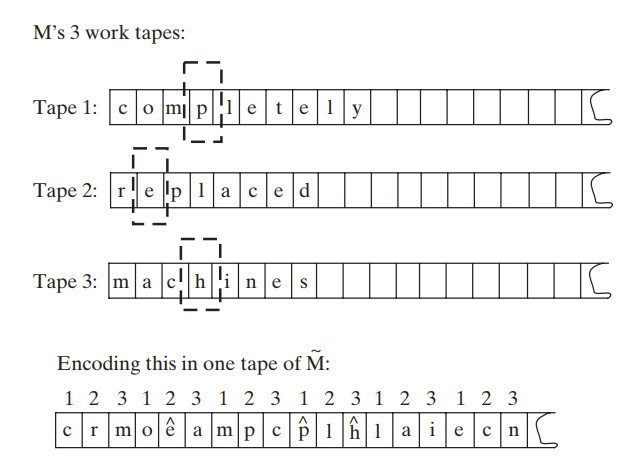
\includegraphics[width=10cm]{s2.png}
\caption{Simulating a machine $M$ with three tapes using a machine $\widetilde{M}$ with a single tape.}
\label{fig:scetch2}
\end{figure}

With a bit of care, one can ensure that the proof of Claim 1.6 yields a TM $\widetilde{M}$ with the following property: Its head movements do not depend on the input but only depend on
the input length. That is, every input $x \in \{0, 1\}^{∗}$ and $i \in \mathcal{N}$, the location of each of $M$’s
heads at the ith step of execution on input $x$ is only a function of $|x|$ and $i$. A machine
with this property is called oblivious, i.e it has following 
